\section{The Compact Muon Solenoid}\label{ch:cms:CMS}

Data used in this thesis were collected by the CMS experiment. CMS is situated at LHC collision Point 5 near Cessy, France, and is depicted in Figure~\ref{fig:cms:cms_full}. CMS was designed for highly performant reconstruction of muons over a wide momentum range, high resolution tracking of charged particles, high energy resolution for electromagnetic processes, and high jet and \met resolution ~\cite{Ball:2007zza,Bayatian:2006nff}. This is achieved by the four primary sub-detector systems---from innermost to outermost---the silicon tracking system, electromagnetic calorimeter, hadronic calorimeter, and the muon system. A detailed cross sectional view of the detector and constituent subsystems is presented in Figure~\ref{fig:cms:cms_quarter}.

\begin{figure}[htb]
\centering
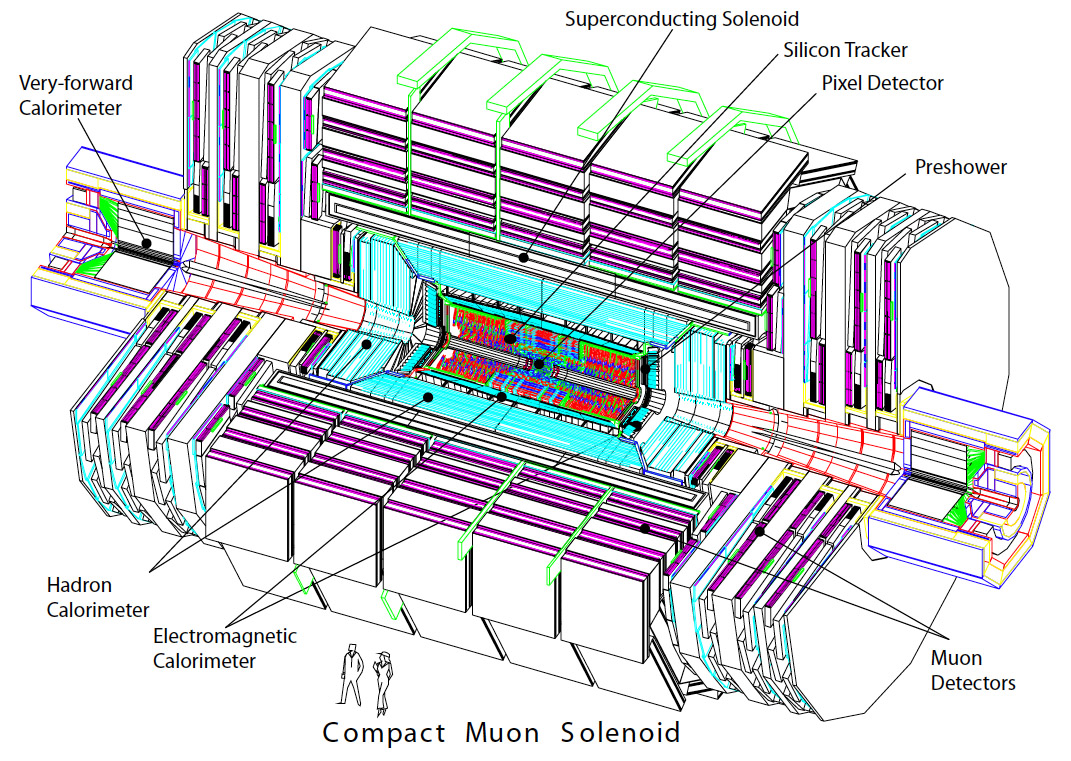
\includegraphics[width=0.75\textwidth]{plots/CMS/cms.png}
\caption{A 3-d cut-away view of the CMS detector, showing the relative position and size of the subdetectors as well as the orientation of the experiment with repsect to the beamline.}
\label{fig:cms:cms_full} 
\end{figure}

\begin{figure}[htb]
\centering
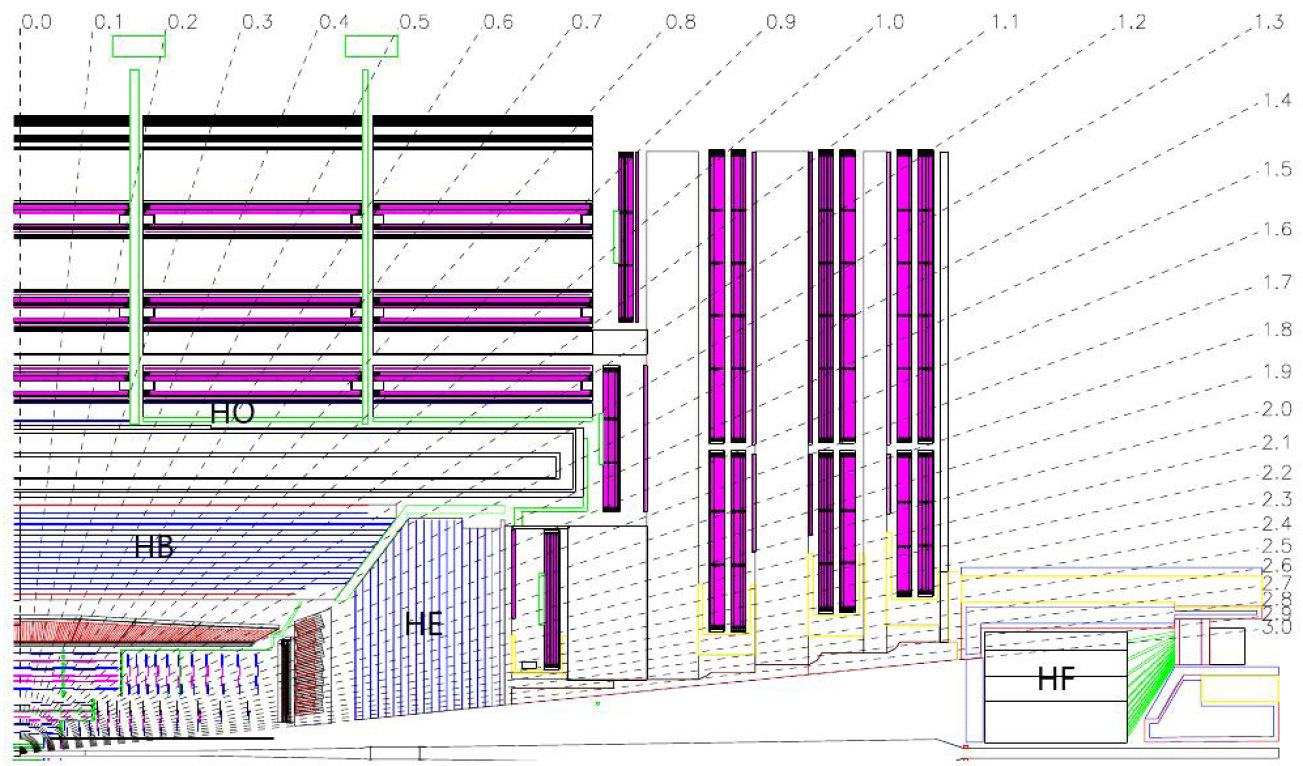
\includegraphics[width=0.75\textwidth]{plots/CMS/cms_quarter.png}
\caption{Quarter-view schematic of the CMS detector showing the arrangement of the subsystems. Radially arranged dotted lines indicate the pseudorapidity ($\eta$) coverage.}
\label{fig:cms:cms_quarter}
\end{figure}

% %% finish section and uncomment
% \subsection{Coordinates \& Units}
% Before describing the detector, an overview of standard terminology for the coordinate system, units, and other commonly used terminology is provided.
% \begin{itemize}
%     \item  rapidity
%     \item $\Delta R = \sqrt{\Delta\eta^2+\Delta\phi^2}$
% \end{itemize}
% % 



\subsection{Magnet}\label{ch:cms:magnet}
The namesake superconducting magnet provides a uniform $|\vec{B}| = 3.8 \,\mathrm{T}$ field at inner radii and a field of $|\vec{B}| = 2 \,\mathrm{T}$ at radii outside of the magnet. This is achieved using a liquid helium-cooled niobium-titanium superconductor mechanically supported by a high-purity aluminum chassis. The operational temperature of the magnet is $T = 4.6 \,\mathrm{K}$, which maintains the current and temperature below the critical values so that $|\vec{B}| = 3.8 \,\mathrm{T}$ field~\cite{Acquistapace:1997fm}.

\begin{figure}[htb]
\centering
  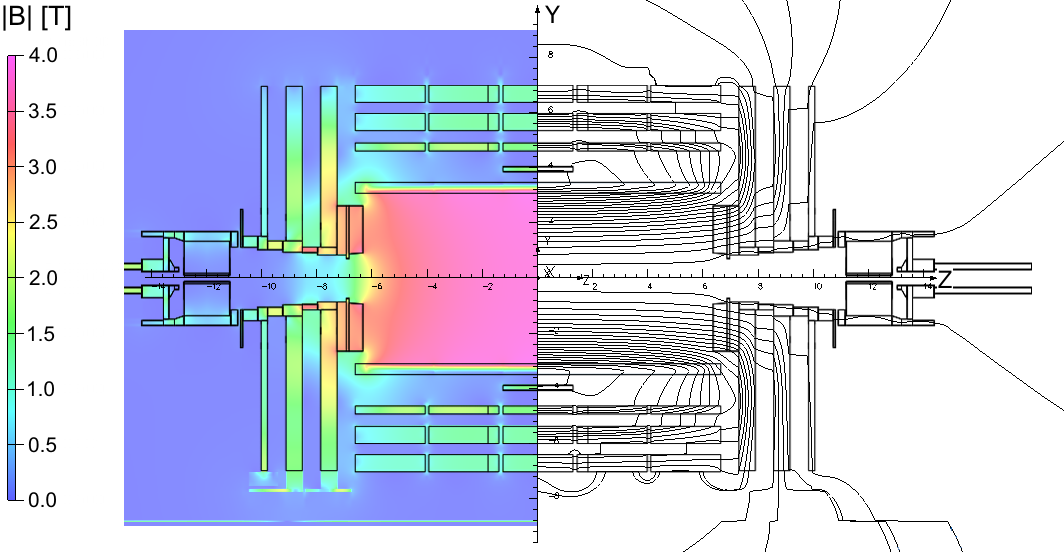
\includegraphics[width=0.9\linewidth]{plots/CMS/magnetic_field.png}
  \caption{Diagram depicting the magnetic field strength and field lines from the CMS superconducting solenoid~\cite{Chatrchyan:2009si}.}
  \label{fig:cms:bfield}
\end{figure}
With an inner radius of 6 meters, the solenoid bore houses the silicon tracker, electromagnetic calorimeter, and the hadronic calorimeter. The solenoid ensures a uniform inner magnetic field of $|\vec{B}| = 3.8 \,\mathrm{T}$ along the $z$-axis for these sub-systems. On the outer radius of the solenoid, muon chambers are interspersed with the steel return yoke. The role of the return yoke is two-fold---extend uniformity and strength of the magnetic field outside of the solenoid and to act as an absorber layer for the muon chambers. 

%%%%%%%%%%%%%%%%%%%%%%%%%%%%%%%%%%%%%%%%%%%%%%%%%%%%%
%                   Tracker 
%%%%%%%%%%%%%%%%%%%%%%%%%%%%%%%%%%%%%%%%%%%%%%%%%%%%%
\subsection{Trackers}\label{ch:cms:tracker}
%% intro and purpose
The innermost detector system is the silicon tracker. The tracker measures the trajectory of charged particles from the collision point, and is designed to provide efficient and high-precision position reconstruction of charged particle trajectories through the tracker volume. In addition to providing high-resolution momentum information, the tracker should be able to identify isolated electromagnetic clusters, as in the $W\rightarrow e\nu$ and $Z \rightarrow ee$ channels, and to separate them from non-isolated electrons\cite{Karimaki:368412}.

%% design considerations
Other design considerations are the proximity of the inner tracker to the collision point and the material budget. Due to its close proximity to the beamline, the tracker is subjected to a high particle flux, with thousands of particles per bunch crossing every $25\,\mathrm{ns}$. This necessitates a radiation-hard detector with fast readout and high granularity to reduce multiple-occupancy per channel. However, the amount of material in the detector---including the supporting electronics, cabling, and cooling systems---increases the amount of bremsstrahlung, which degrades the resolution of isolated electron measurements. Therefore the amount of detector material also needs to be minimized.

Given these design and operational considerations, the tracker uses silicon technology in the form of pixel and strip detectors. The silicon pixels are a p-n junction operated under a reverse-bias voltage. Charged particles traversing the depletion zone create electron-hole pairs, which drift under the reverse-bias and are collected by readout electronics.

%% design/construction
%% Pixel detector
The inner tracking system is composed of a silicon pixel detector, with 3 layers of pixels in the barrel ($r=4.4 \,\mathrm{cm}$, $7.3 \,\mathrm{cm}$, and $10.2 \,\mathrm{cm}$, $\mathrm{length}=53\,\mathrm{cm}$) and 2 layers of pixels in the end-cap region (inner radius of 6 cm, outer radius 15 cm, located at $|z|=34.5 \,\mathrm{cm}$ and $|z|= 46.5 \,\mathrm{cm}$). The individual pixels are 150x100$\mu\mathrm{m}$, with 60 million pixels, where the fine segmentation is intended to minimize track occupancy per channel. A schematic depicting the geometry of the inner and outer tracking systems is shown in Figure~\ref{fig:cms:tracker}

%Strip Detector

Surrounding the inner tracker, the outer tracker is a series of silicon strip detectors. The tracker inner barrel (TIB) covers $20 \,\mathrm{cm} < r < 55 \,\mathrm{cm}$, and an additional six-layer outer barrel (TOB) extending to $r<116cm$.  The TIB spans $\pm$ 80 cm and TOB spans $\pm$ 118 cm in $z$. 
Tracker disk segments with strips arranged in rings are located within the inner radius of the TOB at $z$ position just outside of the TIB. Further nine endcap ring layers are positioned beyond the $z$ extent of the TOB, between $z=\pm$95.2cm and $\pm$ 264cm. Depending on the position, each layer contains between 2 and 7 rings of detector with inner radius 21.8cm-39cm and outer radius 60.8cm.\phil{mention TEC}

\begin{figure}[htb]
\centering
  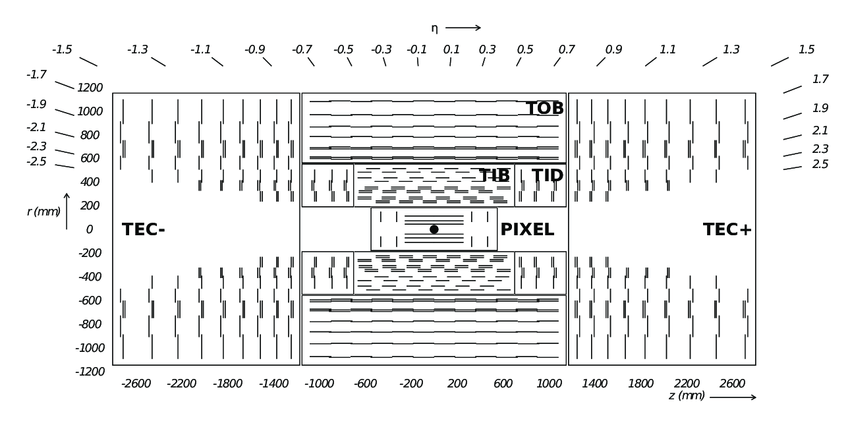
\includegraphics[width=0.7\linewidth]{plots/CMS/r-z-slice-of-the-CMS-Tracker.png}
  %https://cds.cern.ch/record/40524
  \caption{Schematic of the CMS tracking system. The silicon pixel detector is surrounded by the inner (TIB) and outer (TOB) barrel strip detectors. The endcap (TEC) strip detectors provide forward coverage up to |$\eta$|<2.5.~ \protect\cite{CMS_tracker_diagram}}
  \label{fig:cms:tracker}
\end{figure}


%%%%%%%%%%%%%%%%%%%%%%%%%%%%%%%%%%%%%%%%%%%%%%%%%%%%%
%                   ECAL 
%%%%%%%%%%%%%%%%%%%%%%%%%%%%%%%%%%%%%%%%%%%%%%%%%%%%%
\subsection{Electromagnetic Calorimetry}\label{ch:cms:ecal}
 % Cite CMS ECAL TDR
%% intro/purpose
The energy carried by electrons and photons is measured by the electromagnetic calorimeter (ECAL). The ECAL is a homogenous and hermetic calorimeter situated just outside of the silicon tracker, which measures the energy carried by electrons and photons.
%% Design  considerations
Driving factors determining the design of the ECAL is the need for a fast response time sufficient for collisions occuring every 25ns as well as a high-resolution measurement necessary for the $H\rightarrow \gamma \gamma$ measurement. To this end, the active material is a scintillating lead tungstate ($\mathrm{PbWO_4}$) crystal. Incident electrons and photons create an electromagnetic shower within the crystal. As the shower propagates, scintillation light is produced by excitations in the crystal lattice caused by the particles in the shower. The scintillation light, proportional to the energy deposited by the incident particle, is collected and read out by a photodiode\cite{CERN-LHCC-97-033}.

\begin{figure}[htb]
\centering
  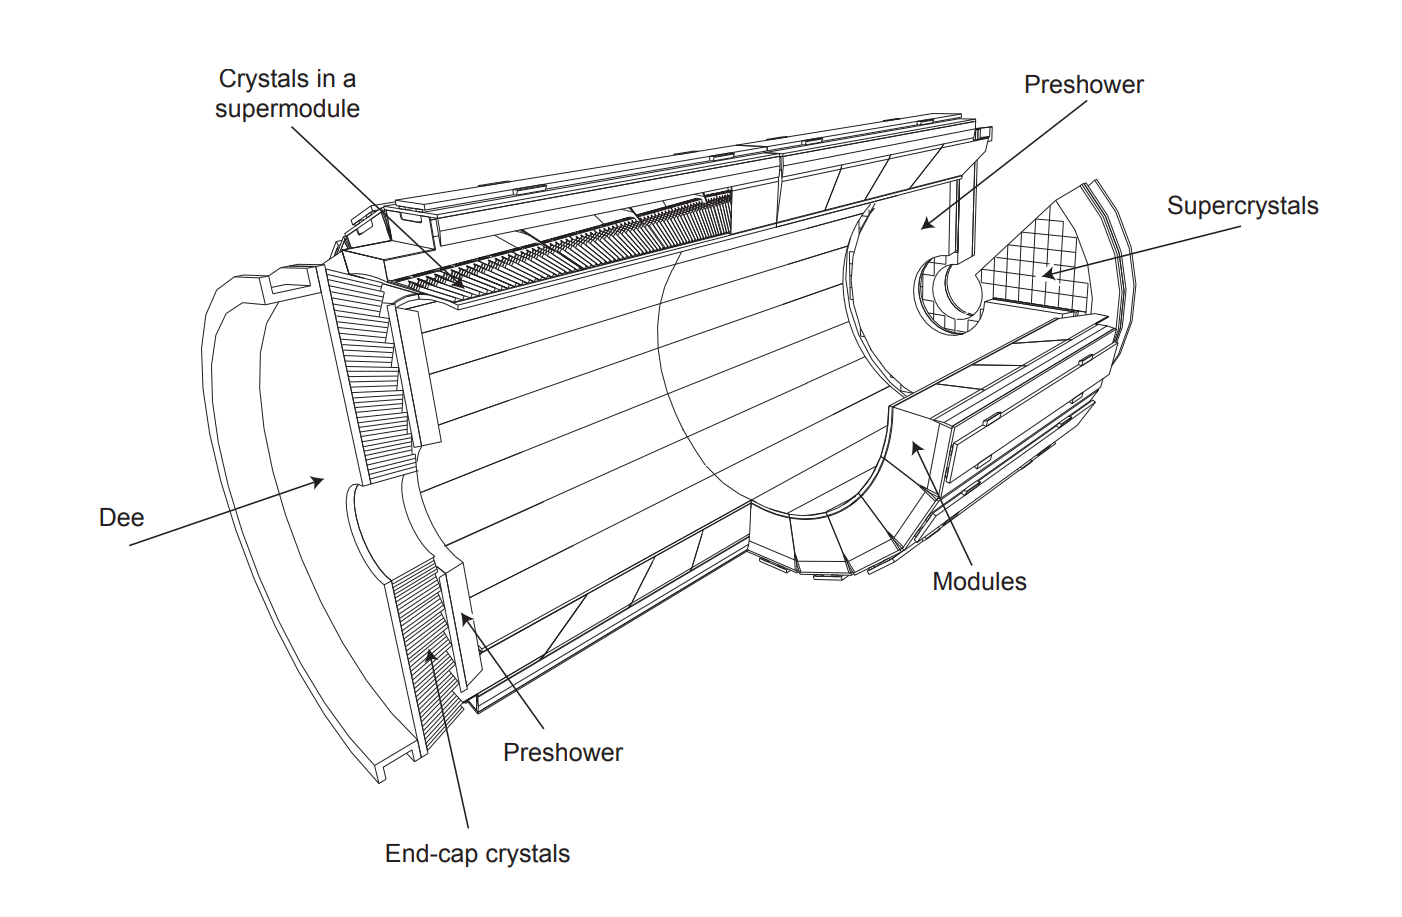
\includegraphics[width=0.9\linewidth]{plots/CMS/ecal_1.PNG}
  %https://cds.cern.ch/record/40524
  \caption{Schematic of the ECAL demonstrating the location and orientation of the crystals in the barrel and endcap. The radial pointing of the crystals is visible.~\protect\cite{Benaglia_2014}}
  \label{fig:cms:ecal1}
\end{figure}

\begin{figure}[htb]
\centering
  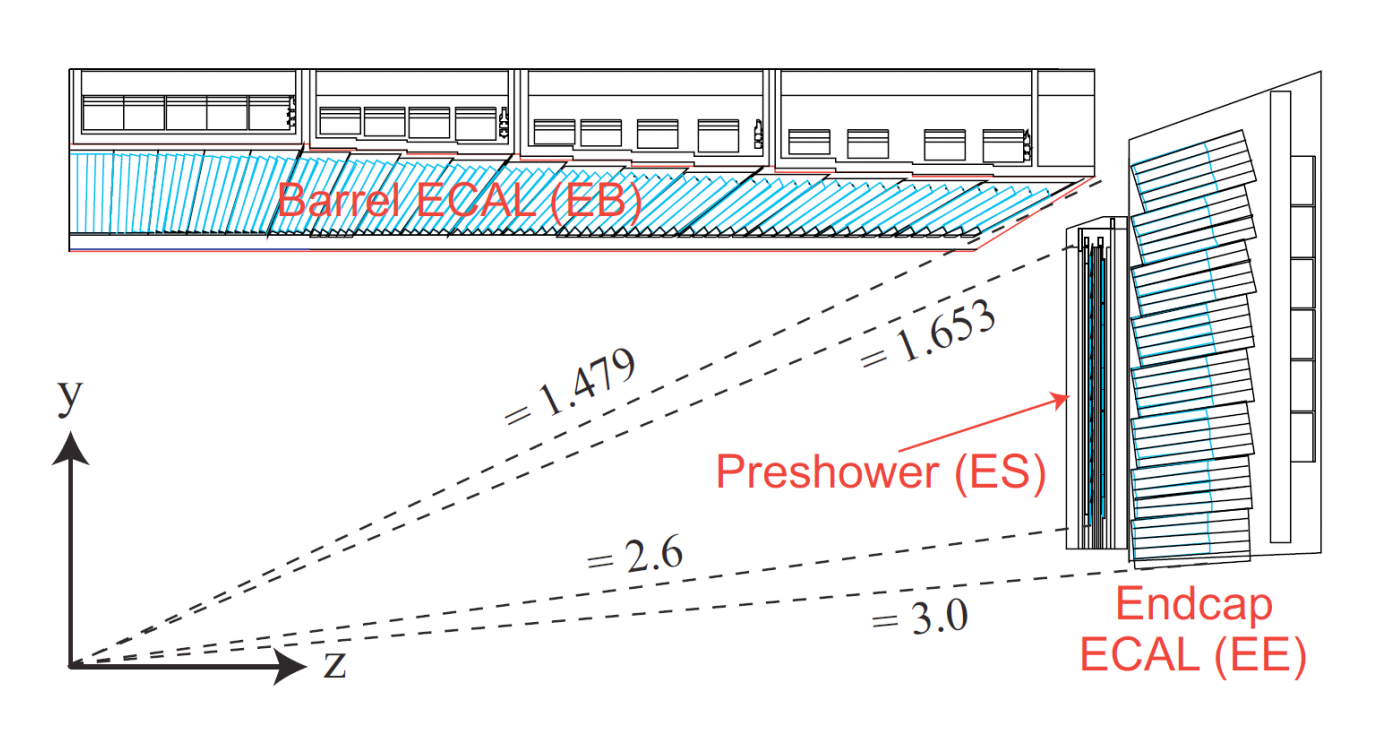
\includegraphics[width=0.7\linewidth]{plots/CMS/ecal_2.PNG}
  %https://cds.cern.ch/record/40524
  \caption{Quarter-view of the ECAL showing the position and orientation of the crystals.~\protect\cite{Benaglia_2014}}
  \label{fig:cms:ecal2}
\end{figure}

In the barrel region, the wedge-shaped crystals (approximately 2.2x2.2x23cm, corresponding to 26 radiation lengths in depth) are arranged radially, covering up to $|\eta|<1.49$. The endcap provides coverage from $1.47<|\eta|<3.0$, with the 3x3x22cm (approximately 25 radiation lengths)  crystals arranged approximately parallel to the beamline. Crystal dimensions are compatible with electromagnetic shower sizes in $\mathrm{PbWO_4}$. The orientation of the crystals depends on their $|\eta|$ position, as they are angled towards $3\deg$ of the collision point, as shown in Figure~\ref{fig:cms:ecal2}.
%% Radiation Damage
 The $\mathrm{PbWO_4}$ crystals are radiation hard, but exposure to radiation damages the crystals, producing color centers which reduce the transparency of the crystal volume. Transparency loss and the associated change in energy response is most prominent in regions of high $|\eta|$ which were subjected to the highest levels of radiation\cite{Cipriani:2018ule}. These defects can anneal during times without collisions. The ECAL is equipped with a laser system which monitors the transparency of the crystals. Calorimeter performance can be maintained by accounting for the transparency loss experienced by indivdiual crystals\cite{CERN-LHCC-97-033}.   

%% capabilities
The ECAL energy resolution is described in Equation~\ref{eq:cms:ecalresolution}. 
\begin{equation}
\frac{\sigma(E)}{E}=\frac{2.8\%}{\sqrt{E}} \oplus \frac{120 MeV}{E} \oplus 0.3\%
\label{eq:cms:ecalresolution}
\end{equation}
The contributions to the energy resolution are, respectively, the stochastic term, electronics noise term, and the constant term. Stochastic term, $2.8\%/\sqrt{E}$, accounts for statistical fluctuations in shower detection, and it is small due to ECAL being a homogenous calorimeter. The constant noise term, $0.3\%$, includes detector calibration and instability\cite{Adzic:2007mi}.
%%%%%%%%%%%%%%%%%%%%%%%%%%%%%%%%%%%%%%%%%%%%%%%%%%%%%
%                   HCAL 
%%%%%%%%%%%%%%%%%%%%%%%%%%%%%%%%%%%%%%%%%%%%%%%%%%%%%
\subsection{Hadronic Calorimeter}\label{ch:cms:hcal}
%% intro/purpose
The Hadronic Calorimeter (HCAL) measures the energy of charged hadrons. 
%% purpose
%% design consideration
%% design/construction

The HCAL has four subsystems---Barrel (HB), Endcap (HE), Outer (HO), and Forward (HF)---with a quarter slice of the detector shown in Figure~\ref{fig:cms:hcal}.  HB, HE, and HO are sampling calorimeters using plastic scintillator and steel and brass absorbers. HB extends from the outside of the ECAL to the inner radius of the solenoid coil: $r=1.77\,\mathrm{m}$ - $r=2.95\,\mathrm{m}$ and covers $|\eta| < 1.3$ with an $\eta-\phi$ segmentation of $0.87\times0.87$. The interior absorber is a $40\,\mathrm{mm}$ thick steel plate, followed by eight layers of $50.5\,\mathrm{mm}$ thick brass plates interleaved with $3.7\,\mathrm{mm}$ thick plastic scintillator tiles, and final steel plate absorber 75mm thick, providing a total interaction length of $5.8\,\lambda_I$. The layers of HO are situated at the outer radius of the solenoid, designed to catch showers for high energy hadrons that are not contained within the other HCAL subsystems. There is an extra HO layer near $|\eta|\approx 0$ where the interaction depth of the HB is shortest. The construction of HB and HE are cylindrically nested alternating layers of brass absorber and scintillator, with the first absorber layer made of steel. The HE extends coverage to $|\eta| < 3$, and consists of 10 layers of alternating scintillator and brass absorber, with a steel first absorber layer.

HF is a sampling calorimeter using quartz fibers embedded in steel. It is situated in the far forward region of the detector, with coverage up to $|\eta| < 5.2$. Due to its position, the HF experiences significantly higher particle flux than the other HCAL subsystems and the HF needed to have extremely fast response and radiation hardness
\cite{CERN-LHCC-97-031}.

\begin{figure}[htb]
\centering
  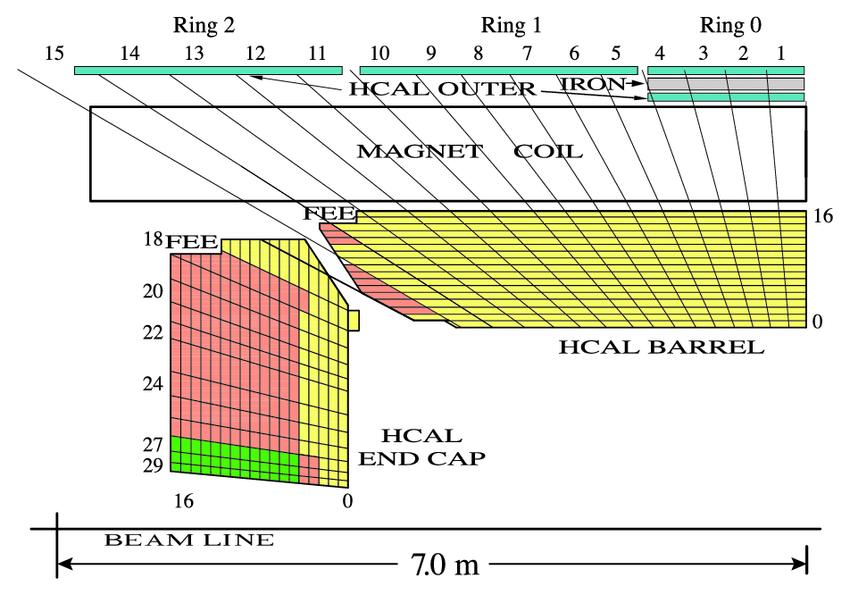
\includegraphics[width=0.7\linewidth]{plots/CMS/HCAL-quarter.png}
  %https://cds.cern.ch/record/40524
  \caption{Quarter-view of the HCAL showing the positioning and segmentation of the barrel, endcap, and outer subsystems.~\protect\cite{Chatrchyan:1223869}}
  \label{fig:cms:hcal}
\end{figure}


The HCAL is a sampling calorimeter. Incident charged hadrons undergo multiple scattering within the absorber material, producing hadronic showers that propagate in the direction of the particles intial trajectory. As the showers develop, they pass through the absorber layer and traverse the scintillator layer, where the particles in the shower induce excitations resulting in scintillation light. The light is wavelength shifted and carried by optical fibers to a photodiode where it is read out and digitized. In the HF, quartz fibers produce Cherenkov light. 



%% capabilities
The energy resolution of the HCAL, described in Equation~\ref{eq:cms:hcal_res} is representative of a sampling calorimeter. Resolution is affected by the limited detector volume available to the HCAL\cite{Cavallari_2011}.

\begin{equation}
\frac{\sigma(E)}{E}=\frac{110\%}{\sqrt{E}} \oplus 7.3\%
\label{eq:cms:hcal_res}
\end{equation}
The stochastic term (${110\%}/\sqrt{E}$) accounts for the statistical fluctuations in shower detection, which is relatively large for the HCAL due to its design as a non-compensating sampling calorimeter. The constant $7.3\%$ term is due to detector calibration limitations.

\subsubsection{HCAL Reconstruction Algorithms}
In HB and HE, the total pulse width from light collection and electronic readout is larger than the 25\ns separation between LHC bunch crossings. Output from the HPD is digitized and integrated in 25\ns-wide bins. Approximately 60\% of the pulse width is contained within the first 25\ns and and 90\% of the pulse is contained within the first 50\ns. LHC Run II conditions with 25\ns separation between bunch crossings potentially produces readout with substantial overlap between pulses generated by interactions from consecutive bunch crossings. An algorithm to perform hit reconstruction in each calorimeter tower was developed for Run II in order to mitigate the effect of out-of-time pileup events on the energy resolution of the HB and HE readout channels. This was achieved by assuming the presence of out-of-time pileup interactions from the immediately precedent and antecedent bunch crossings. A fitting template is constructed out of 3 HCAL pulse shape templates, where the free parameters are the arrival times and normalizations of each pulse as well as a floating baseline to accommodate noise. The resulting normalization of the in-time pulse determines the energy for the reconstructed hit in each channel. 
%% do i have a diagram demonstrating the fits
In addition to providing the offline HCAL hit reconstruction, the algorithm is used in HCAL operations and data validation. In addition to hit energy, the fitting procedure determines the arrival time with a resolution of 1\ns. This provides the ability to monitor and calibrate the relative timing of the channels in HB and HE. 
%%%%%%%%%%%%%%%%%%%%%%%%%%%%%%%%%%%%%%%%%%%%%%%%%%%%%
%                   Muon 
%%%%%%%%%%%%%%%%%%%%%%%%%%%%%%%%%%%%%%%%%%%%%%%%%%%%%
\subsection{Muon System}\label{ch:cms:muons}
%% intro/purpose
The outermost detector system is the muon chambers. Situated around the return yoke, the muon detectors are used for muon triggering, muon identification, and muon momentum measurement. Particles that make it through CMS and reach the muon systems are almost exclusively muons. Muon detector information is combined with tracking information to enhance muon reconstruction.
The muon system uses three detector technologies: resistive plate chambers (RPC), drift tubes (DT), and cathode strip chambers (CSC)\cite{CMS:1997iti}. 
% blahhhh

The barrel region technology is drift tubes, with coverage up to $|\eta| < 1.2$. These are suitable due to the fairly uniform magnetic field and low particle flux. The barrel region is constructed of four cylindrically nested sets of rectangular drift tube components, with 12 segments in $\phi$, and panels at each radius grouped to form a muon station. The stations are located in alternating layers with the magnetic field return yoke. Each station consists of 8 layers of drift tubes. The arrangement of the barrel muon stations can be seen in Figure~\ref{fig:cms:muons}. The drift chambers containing a $\mathrm{CO_2}$/Argon gas mixture, which has a drift velocity of 55 $\mu$m/ns (about 400ns maximum drift time) \cite{Chatrchyan:2013sba}.
\begin{figure}[htb]
\centering
  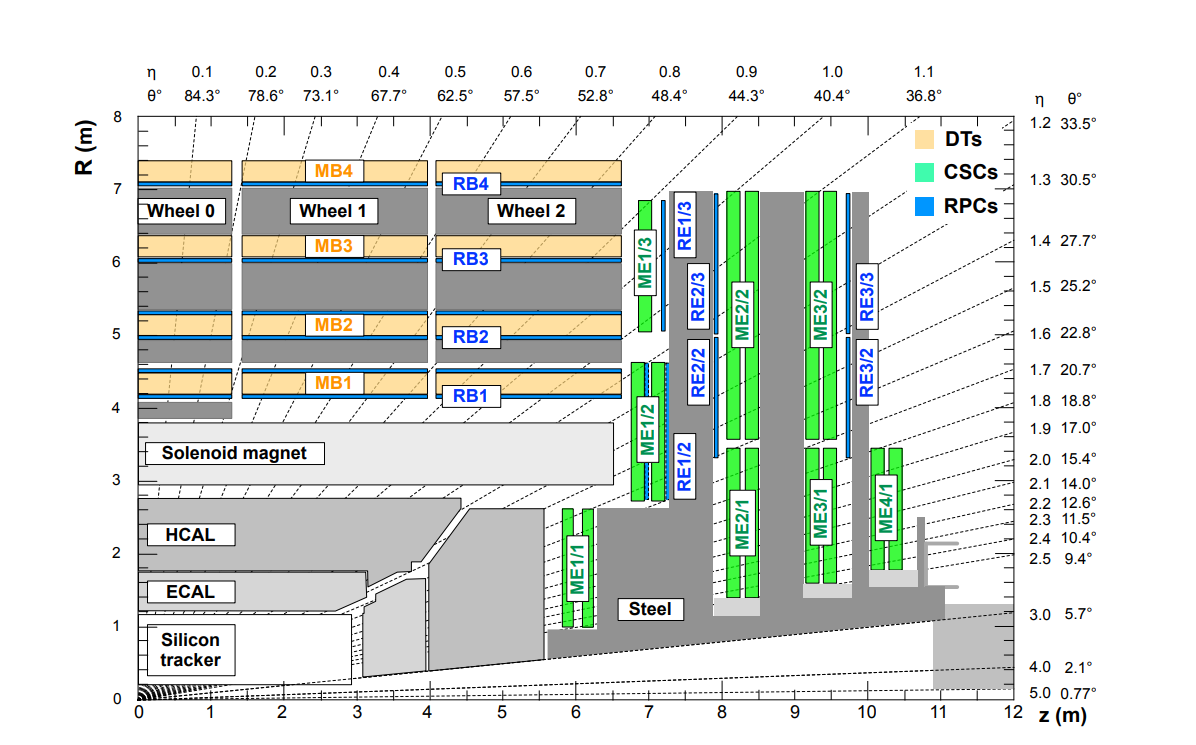
\includegraphics[width=0.7\linewidth]{plots/CMS/cmsmuon.png}
  \caption{Quarter-view of the CMS muon system illustrating the position of the DT, CSC, and RPC detectors within the magnetic field return apparatus \protect\cite{Chatrchyan:2013sba}.}
  \label{fig:cms:muons}
\end{figure}


%% design/construction
The endcap muon detectors use a cathode strip chamber (CSC). CSC are multi-wire proportional chambers with a cathode strip as the readout and can provide a precise location of ionization. The endcap stations are grouped by $z$ position, covering $1.2 < |\eta| < 2.4$. CSCs are used in the endcap regions because their high granularity and short drift distance makes them more suitable for the higher event rate and non-uniform magnetic field in this region. The CSC strips are arranged radially, and contain 6 layers which each provide a 2-coordinate hit position in the $r-\phi$ plane. Additional readout is taken from the anode wires, which provide a rough position meaurement in $r$.
%% RPC trigger
In addition to the CSC and DT which provide full $\eta$ coverage up to $|\eta| < 2.4$, the muon system also utilizes a set of resistive plate chambers as an independent trigger system. The RPCs cover $|\eta| < 1.6$, and are a double-gap system operated in avalanche mode. The RPCs have poor position resolution, but have a response time of 1 ns and can be used to measure correct bunch crossing time at the highest LHC luminosities. 
